\documentclass[
journal=jctcce,
layout=twocolumn
]{achemso}

\setkeys{acs}{
	abbreviations = false,
	articletitle  = false,
	keywords      = false,
	maxauthors    = 10,
	super         = true
}

% Comment below before submitting
\let\titlefont\undefined
\usepackage[fontsize=11pt]{scrextend}
\usepackage[hidelinks,colorlinks,citecolor=blue]{hyperref}
%\flushbottom
% Comment above before submitting

\usepackage{threeparttable}
\usepackage{amsmath}
\usepackage{amssymb}
\usepackage[T1]{fontenc}
\usepackage[table]{xcolor}
\definecolor{lightgray}{gray}{0.9}

\newcommand{\mt}[1]{\boldsymbol{\mathbf{#1}}}   % matrix symbol
\newcommand{\vt}[1]{\boldsymbol{\mathbf{#1}}}   % vector symbol
\newcommand{\tr}[1]{#1^\text{t}}                % transposition
\newcommand{\diff}[2]{\frac{\partial #1}{\partial #2}} % derivative
%\newcommand{\diff}[2]{\nabla_{#2}#1}            % derivative
\newcommand{\sdiff}[2]{\nabla^2_{#2}#1}         % 2nd derivative
\newcommand{\Ham}[1]{{\mathcal H}_\text{#1}}    % Hamiltonian
\newcommand{\Liu}[1]{i\!L_\text{#1}}            % Liouville
\newcommand{\timestep}{h}
\newcommand{\modified}[1]{\widetilde{#1}}

\usepackage{array}
\newcolumntype{L}{>{$}l<{$}}
\newcolumntype{C}{>{$}c<{$}}
\newcolumntype{R}{>{$}r<{$}}

\newenvironment{smallarray}[1]                          % small arrays
{\null\,\vcenter\bgroup\scriptsize
	\renewcommand{\arraystretch}{1.5}
	\arraycolsep=.13885em
	\hbox\bgroup$\left[\array{@{}#1@{}}}
{\endarray\right]$\egroup\egroup\,\null}
\listfiles

\author{Ana J.
Silveira}
\email{asilveira@plapiqui.edu.ar}
\affiliation{Planta Piloto de Ingenier\'ia Qu\'imica, PLAPIQUI, Universidad Nacional del Sur, Camino La Carrindanga Km 7-CC: 717, Bah\'ia Blanca, Argentina}

\author{Charlles R.
A.
Abreu}
\email{abreu@eq.ufrj.br}
\affiliation{Chemical Engineering Department, Escola de Qu\'imica, Universidade Federal do Rio de Janeiro, Rio de Janeiro, RJ 21941-909, Brazil}

%\title{Revisiting the Nos\'{e}-Hoover chain thermostat for Rigid-Body Molecular Dynamics}
\title{Improvement of Deterministic NVT Molecular Dynamics via Backward Error Analysis}

%\abbreviations{AAA, BBB, CCC}
\keywords{aaa, bbb, ccc}

\begin{document}

\begin{tocentry}
	Graphical Abstract
\end{tocentry}

\begin{abstract}
	Abstract.
\end{abstract}

\section{Introduction}

Molecular Simulation, being the computational realization of Statistical Mechanics \cite{Tuckerman_2010}, involves several types of approximations in order to mimic ``real'' physical systems.
Naively, one would expect those approximations to only produce quantitative deviation from experimental values, and usually we tend to attribute any disagreement to a lack of accuracy of the force field.
However, what can be hidden in the deviations are actually systematic errors, which may introduce non-physical behavior.
For instance, it has already been shown that the unavoidable truncation errors, associated with the numerical integration in Molecular Dynamics (MD), disrupt the equipartition of kinetic energy and, as a consequence, the temperature becomes an undefined property \cite{Eastwood_2010}.
In a previous paper \cite{Silveira_2017}, we reported the same artifact to occur on the partition of kinetic energy between translational and rotational degrees of freedom in rigid-body MD.
That finding brings into question the method introduced by Kamberaj and co-workers \cite{Kamberaj_2005} which, assuming equipartition, couples separate chains of Nos\'{e}-Hoover thermostats on the rotational and translational degrees of freedom, but fails to reproduce the specified temperature for certain time step sizes.

The relevance of rigid-body MD stems from the fact that not only some molecules are modelled as rigid bodies, like the ubiquitous case of water,\cite{Jorgensen_1983} but also it is a simple coarse-graining strategy for systems that might be designed as collection of interconected rigid bodies, like proteins and nanoparticules \cite{Knorowski_2012, Patra_2013}.
As a matter of fact, the approach of \citeauthor{Kamberaj_2005} \cite{Kamberaj_2005}, which is implemented, for instance, in the softwares packages HOOMD-\textit{blue} \cite{Anderson_2008} and LAMMPS \cite{Plimpton_1995}, has been applied to simulate small molecules,\cite{Geiger_2013, Aimoli_2014, Aimoli_2014_2} as well as membranes \cite{Bucior_2012}, molecular motors \cite{Akimov_2012}, micelles \cite{Yan_2008} and nanoparticles \cite{Patra_2014}.

The Nos\'{e}-Hoover chain thermostat \cite{Martyna_1992}, routinely used in MD, is based on the extended phase-space approach that includes both the system of interest and extra degrees of freedom, which in turn are intended to control the kinetic energy fluctuations of the physical variables.
The dynamics of those extra degrees of freedom introduces non-Hamiltonian components to the equations of motion, with which backward error analysis is no longer feasible.
Altough it is not possible to devise symplectic integrators, one can rigurously obtain measure-preserving numerical solvers \cite{Sergi_2001, Ezra_2004, Ezra_2006}.

In this paper, we derive time reversible and measure-preserving numerical integrators for rigid-body MD in the canonical (NVT) ensemble.
The starting point is our previous work on the microcanonical (NVE) ensemble \cite{Silveira_2017}, which employs the unit quaternion representation for the rotational degrees of freedom.
Simultaneosuly coupling the translational and rotational degrees of freedom to a unique Nos\'{e}-Hoover chain thermostat, we are able to mantain the temperature of the system at its specified value.
The analysis of the integrators includes comparisons with results from the method introduced by \citeauthor{Kamberaj_2005} \cite{Kamberaj_2005}, as well as with the Hybrid Monte Carlo (HMC) method,\cite{Duane_1987} which is exact in the sense that truncation errors do not affect its accuracy.
We also include results from simulations using the conventional SHAKE \cite{Ryckaert_1977} procedure, also coupled to a unique Nos\'{e}-Hoover chain.

The paper is organized as follows.
In Sec.~\ref{sec:theory} we briefly review the equations of motion in the NVE ensemble, which are the basis for developing the corresponding dynamics in the NVT ensemble.
In Sec.~\ref{sec:numerical_solvers} we devise the corresponding numerical integrators, whose performance and correctness we assess in Sec.~\ref{sec:numerical_results}.
Finally, we present some concluding remarks in Sec.~\ref{sec:conclusion}.

\section{Proposed Methodology}
\label{sec:methodology}

\subsection{NVE Dynamics: Notation and Symplectic Integration}

In a previous paper \cite{Silveira_2017}, we took advantage of a particular factorization of the orientation matrix expressed in terms of quaternion components to
1) derive a new exact solution for torque-free rotations and use it as part of a symplectic numerical integrator for the motion of rigid bodies and
2) reinterpret the approximate NO-SQUISH method \cite{Miller_2002} as a sequence of uniform rotations around the principal axes of a body, thus unveiling its equivalence to a method previously developed by Dullweber and co-workers \cite{Dullweber_1997}.

The Hamiltonian system of ordinary differential equations (ODE) that describes a rigid-body motion are \cite{Silveira_2017}
\begin{subequations}
	\label{eq:ODE system for NVE}
	\begin{align}
%
	&\dot{\vt r} =
	%+\diff{\Ham{}}{\vt p} =
	{\mt M}^{-1} {\vt p}, \\
%
	&\dot{\vt p} =
	%-\diff{\Ham{}}{\vt r} = 
	{\vt F}, \\
%
	&\dot{\vt q} =
	%+\diff{\Ham{}}{\vt \pi} =
	\frac{1}{2} \mt B(\vt q) \vt \omega, \text{ and} \label{eq:EDO_q} \\
%
	&\dot{\vt \pi} =
	%-\diff{\Ham{}}{\vt q} =
	\frac{1}{2} \mt B(\vt \pi) \vt \omega + 2 \mt C(\vt q) \vt \tau, \label{eq:EDO_pi}
	\end{align}
\end{subequations}
with $\vt \omega = \frac{1}{2} {\mt I}^{-1} \tr{\mt B}(\vt q) {\vt \pi}$.
In these equations, $\vt r$ is the center-of-mass position of the body, $\vt p$ is its linear momentum, $\vt q$ is a unit quaternion that determines its orientation, and $\vt \pi$ is the conjugated momentum of such quaternion.
Vectors $\vt F$ and $\vt \tau$ are, respectively, the resultant force and resultant torque exerted on the body, both represented in the space-fixed frame of reference, while $\vt \omega$ is the three-dimensional angular velocity.
Matrices $\mt M$ and $\mt I$ are diagonal ones.
The former contains the body mass in all three diagonal entries while the latter contains the three principal moments of inertia.
Finally, the matrix-valued functions $\mt B$ and $\vt C$ are defined as
\begin{equation*}
\label{eq:def_B_and_C}
\mt B(\vt q) = \begin{smallarray}{rrrr}
-q_2 & -q_3 & -q_4 \\
 q_1 & -q_4 &  q_3 \\
 q_4 &  q_1 & -q_2 \\
-q_3 &  q_2 &  q_1
\end{smallarray}
%
\; \text{and} \;
%
\mt C(\vt q) = \begin{smallarray}{rrrr}
-q_2 & -q_3 & -q_4 \\
 q_1 &  q_4 & -q_3 \\
-q_4 &  q_1 &  q_2 \\
 q_3 & -q_2 &  q_1
\end{smallarray}.
\end{equation*}

The position of any constituent particle $j$ of a rigid body will vary with time according to $\vt R_j(t) = \vt r(t) + \tr{\mt A}(\vt q(t))\vt d_j$, where $\vt d_j$ is the (constant) position of particle $j$ in the body-fixed frame of reference and ${\mt A}(\vt q)$ is the orientation matrix of the body (that is, the rotation matrix connecting the body-fixed and space-fixed frames) expressed as a function of the quaternion components.
The factorization mentioned above, which played a central role in Ref.~\citenum{Silveira_2017}, is as simple as ${\mt A}(\vt q) = \tr{\mt B}(\vt q) {\mt C}(\vt q)$.

The Hamiltonian conserved by Eq.~\eqref{eq:ODE system for NVE} is
\begin{equation}
\label{eq:Hamiltonian}
\Ham{} = K(\vt p, \vt q, \vt \pi) + U(\vt r,\vt q),
\end{equation}
where $K$ and $U$ are the kinetic and potential energies of the body, respectively.
While $U(\vt r, \vt q)$ is an arbitrary function, the kinetic energy is given by
\begin{equation}
\label{eq:kinetic energy}
K = \frac{1}{2} \tr{\vt p} {\mt M}^{-1} {\vt p} + \frac{1}{8} \tr{\vt \pi} {\mt B}(\vt q) {\mt I}^{-1} \tr{\mt B}(\vt q) {\vt \pi}.
\end{equation}

An advantage of this notation is that Eqs.~\eqref{eq:ODE system for NVE} to \eqref{eq:kinetic energy} can also represent a system of $N$ interacting rigid bodies if we consider that vectors $\vt r$, $\vt p$, $\vt q$, and $\vt \pi$ contain the corresponding properties of all bodies piled together.
The same occurs for diagonal matrices $\mt M$ and $\mt I$, whose sizes increase to $3N \times 3N$ in this case.
In addition, $\mt B(\vt q)$ and $\mt C(\vt q)$ become block-diagonal matrices with $4N$ rows and $3N$ columns.
Yet, the notation can be made even more general if $\vt r$, $\vt p$, and $\mt M$ are enlarged further to accommodate a number of freely moving atoms.

A numerical solution of Eq.~\eqref{eq:ODE system for NVE} is usually represented by a stepwise application of the classical time-evolution propagator \cite{Tuckerman_2010} $e^{\timestep \Liu{\tiny NVE}}$ to the system configuration, where $\timestep$ is the time step size and $\Liu{\tiny NVE}$ is the Liouville operator associated to $\Ham{}$.
A symplectic, time-reversible integrator can be devised by splitting the exponential operator according to the Trotter-Suzuki formula \cite{Trotter_1959, Suzuki_1976}
\begin{equation}
\label{eq:splitting NVE}
e^{\timestep \Liu{\tiny NVE}} = e^{\frac{\timestep}{2} \Liu{B}} e^{\timestep \Liu{A}} e^{\frac{\timestep}{2} \Liu{B}} + \mathcal{O}(\timestep^3),
\end{equation}
where $\Liu{A} + \Liu{B} = \Liu{\tiny NVE}$.
In the Verlet-type splitting of Ref.~\citenum{Silveira_2017}, the action of propagator $e^{\frac{\timestep}{2} \Liu{B}}$ is a kick in the linear and quaternion momenta given by ${\vt p} = {\vt p}^\ast + \frac{\timestep}{2} {\vt F}^\ast$ and ${\vt \pi} = {\vt \pi}^\ast + \timestep {\mt C}({\vt q^\ast}) {\vt \tau}^\ast$, respectively, where the asterisk denotes the state immediately before the propagation occurs.
The action of $e^{\timestep \Liu{A}}$ is a simultaneous uniform translation (${\vt r} = {\vt r}^\ast + \timestep {\mt M}^{-1} {\vt p}^\ast$) and torque-free rotation over a full time step.

Brief description of analytical and NO-SQUISH rotations...

\subsection{NVT Dynamics with a Single Thermostat Chain}

Here we propose a new method for simulating a system of rigid bodies in the canonical ensemble.
For this, we couple a single Nos\'{e}-Hoover thermostat chain \cite{Martyna_1992} to all translational and rotational degrees of freedom of the rigid-body system.
This is simpler than the approach of Kamberaj \textit{et al}.,\cite{Kamberaj_2005} who employed separate thermostat chains to these two classes of movement.
To this end, we consider an extra generalized coordinate $\eta_j$ and its conjugate momentum $p_{\eta_j}$ for each thermostat $j$, with $1 \leq j \le M$.
The flow in the extended phase-space no longer conserves the Hamiltonian $\Ham{}$, but an ``extended energy'' given by \cite{Martyna_1992}
\begin{equation}
\label{eq:nvt extended energy}
H = K + U + {\textstyle\sum\limits_{j=1}^{M}} \frac{p_{\eta_j}^2}{2Q_j} + L k_\text{\tiny B} T\eta_1 + k_\text{\tiny B} T {\textstyle\sum\limits_{j=2}^{M}} \eta_j,
\end{equation}
where $k_\text{\tiny B}$ is the Boltzmann constant, $T$ is the system temperature, $L$ is a constant to be determined, and each $Q_j$ is an inertial parameter.
As recommended in Ref.~\citenum{Martyna_1992}, we can make $Q_1 = L k_\text{\tiny B} T t_d^2$ and $Q_j = k_\text{\tiny B} T t_d^2$ for $j \geq 2$, where $t_d$ is a characteristic time scale of the thermostat chain.

Knowledge on the dynamics and statistical mechanics of non-Hamiltonian systems has advanced considerably in recent years.\cite{Tuckerman_1999, Tuckerman_2001, Sergi_2001, Sergi_2003, Ezra_2004, Sergi_2004, Ezra_2006, Sergi_2010_2} Invaluable tools have been devised for the development and analysis of extended phase space methods.
By employing the method of Sergi and Ferrario \cite{Sergi_2001}, we obtain the equations of motion for the NVT dynamics with a single thermostat chain, which are
\begin{subequations}
	\label{eq:ODE system for NVT}
	\begin{align}
%
\label{eq:nhc_r}
	&\dot{\vt r} =
	{\mt M}^{-1} {\vt p}, \\
%
\label{eq:nhc_p} 
	&\dot{\vt p} =
	{\vt F} - \alpha_1 {\vt p},\\
%
\label{eq:nhc_q}
	&\dot{\vt q} =
	\frac{1}{2} \mt B(\vt q) \vt \omega, \\
%
\label{eq:nhc_pi}
	&\dot{\vt \pi} =
	\frac{1}{2} \mt B(\vt \pi) \vt \omega + 2 \mt C(\vt q) \vt \tau - \alpha_1 {\vt \pi}, \\
%
\label{eq:nhc_eta}
	&\dot{\eta}_j = \alpha_j, \text{ and} \\
%
\label{eq:nhc_p_eta}
	&{\dot p}_{\eta_j} = G_j - \alpha_{j+1} p_{\eta_j} \qquad \text{for} \quad 1 \leq j \le M.
	\end{align}
\end{subequations}

In these equations, $\alpha_j$ $=$ ${p_{\eta_j}}/{Q_j}$ for $1 \leq j \le M$ and $\alpha_{M+1} = 0$, while $G_j$ is a generalized force acting on thermostat $j$, defined as
\begin{subequations}
\begin{align}
\label{eq:generalized force NVT}
&G_1 = \tr{\vt p} \diff{K}{\vt p} + \tr{\vt \pi} \diff{K}{\vt \pi} - L k_\text{\tiny B} T \quad \text{and}\\
&G_j = \frac{p_{\eta_{j-1}}^2}{Q_{j-1}} - k_\text{\tiny B} T  \qquad \text{for} \quad j > 1.
\end{align}
\end{subequations}

With $K$ defined as in Eq.~\eqref{eq:kinetic energy}, it turns out that $G_1 = 2K - L k_\text{\tiny B} T$.
It is worth noting that the $\eta$ coordinates are driven variables with no influence on the dynamics, but are often computed for checking how well a numerical integrator conserves $H$.
Analysis of the probability distribution generated by Eq.~\eqref{eq:ODE system for NVT} can be done through the generalized phase-space analysis of Tuckerman \textit{et al}.\cite{Tuckerman_2001} For this, conservation laws must be identified and driven variables eliminated.
If there are no external forces, the vector quantity $e^{\eta_1}\sum_{i=1}^N {\vt p}_i$ and the extended energy $H$ are integrals of motion, while the system's center-of-mass position can be considered as a driven variable,\cite{Tuckerman_2001} such as the $\eta$ coordinates.
Moreover, $2N$ equations must be eliminated due to the constraints involving $\vt q$ and $\vt \pi$.
In the general case, by taking all these facts into account and applying the analysis of Ref.~\citenum{Tuckerman_2001}, we can deduce that the correct canonical distribution is attained if one makes $L = 6N$.
In the particular situation in which one sets $\sum_{i=1}^N {\vt p}_i = \vt 0$ at the onset of a simulation, one must make $L = 6N - 3$ \cite{Martyna_1994}.

\subsection{Measure-Preserving Integration for the NVT Dynamics}

As in the Hamiltonian case, it is possible to devise a splitting scheme for solving Eq.~\eqref{eq:ODE system for NVT} numerically \cite{Tuckerman_2010}.
Ezra \cite{Ezra_2006} introduced a systematic method for deriving accurate integrators which preserve the phase-space measure associated with the original equations of motion.
In short, a splitting scheme will preserve a given measure if each individual propagator does it as well.
By defining a propagator $e^{\timestep \mathcal{L}_\text{\tiny NVT}}$, where $\mathcal{L}_\text{\tiny NVT}$ is a generalized (i.e.
non-Hamiltonian) Liouville operator, the splitting goes as
\begin{equation}
\label{eq:splitting NVT}
e^{\timestep \mathcal{L}_\text{\tiny NVT}} = e^{\frac{\timestep}{2} \mathcal{L}_\text{\tiny NHC}} e^{\timestep \Liu{\tiny NVE}} e^{\frac{\timestep}{2} \mathcal{L}_\text{\tiny NHC}} + \mathcal{O}(\timestep^3),
\end{equation}
where $\Liu{\tiny NVE}$ is the same operator of the previous case and $\mathcal{L}_\text{\tiny NHC}$ aggregates all new terms introduced by the Nos\'e-Hoover chain.
Of course, the NVE part can be integrated exactly as described before.
The NHC part, in turn, can be split even further as
\begin{equation*}
e^{\frac{\timestep}{2} \mathcal{L}_\text{NHC}} = \left[ \left( \textstyle\prod\limits_{j=M}^1 e^{\frac{\timestep}{4n} \mathcal{L}_j }\right) e^{\frac{\timestep}{2n} \mathcal{L}_0 } \left(  \textstyle\prod\limits_{j=1}^M e^{\frac{\timestep}{4n} \mathcal{L}_j }\right)  \right]^n.
\end{equation*}

In the scheme above, the first propagator to act is $e^{\frac{\timestep}{4n} \mathcal{L}_M}$, which promotes a kick in the momentum of thermostat $M$ expressed as $p_{\eta_M} = p_{\eta_M}^\ast + G_M^\ast \frac{\timestep}{4n}$.
Then, propagators $e^{\frac{\timestep}{4n} \mathcal{L}_j}$ act sequentially, with $j$ varying from $M-1$ down to $1$.
With $\phi(x) = \frac{1-e^{-x}}{x}$, the effect of each one is translated as
\begin{align*}
&p_{\eta_j} = p_{\eta_j}^\ast + \Big( G_j^\ast - \alpha_{j+1}^\ast p_{\eta_j}^\ast \Big) \phi\left(\frac{\alpha_{j+1}^\ast \timestep}{4n}\right) \frac{\timestep}{4n} \; \text{and} \\
&\eta_{j+1} = \eta_{j+1}^\ast + \alpha_{j+1}^\ast \frac{\timestep}{4n}.
\end{align*}

After that, propagator $e^{\frac{\timestep}{2n} \mathcal{L}_0}$ establishes the effect of thermostat $1$ on the motion of the rigid bodies, as well as the evolution of coordinate $\eta_1$.
Its action is expressed as ${\vt p} = e^{-\alpha_1^\ast \frac{\timestep}{2n}} {\vt p}^\ast$, ${\vt \pi} = e^{-\alpha_1^\ast \frac{\timestep}{2n}} {\vt \pi}^\ast$, and $\eta_1 = \eta_1^\ast + \alpha_1^\ast \frac{\timestep}{2n}$.
Finally, propagators $e^{\frac{\timestep}{4n} \mathcal{L}_j}$ are applied once again, but now with index $j$ ascending from $1$ to $M$.

For having a low computational cost, the whole procedure described above can be repeated $n$ times with little impact on the overall integration effort, making it feasible to increase the time step $\timestep$ without degrading the accuracy of the NHC part.
In contrast, evaluating the NVE part is expensive for involving force/torque computations and, in addition, its accuracy goes down very quickly as $\timestep$ increases \cite{Davidchack_2010, Silveira_2017}.
A high-order integration scheme\cite{Omelyan_2007, Van_zon_2008} could possibly admit larger time steps, but it would raise both cost and complexity for entailing the computation (or numerical estimation) of force/torque gradients.
The processed splitting approach \cite{Omelyan_2008} seems promising, but its extension to the NVT case without doing back-and-forth processing at every time step would require further theoretical development.
Here we choose to take a simpler path.
Instead of trying to increase accuracy in the evaluation of $e^{\timestep \Liu{\tiny NVE}}$, we attempt to quantify the implied deviations, with which we can both tune the thermostatting procedure and properly weight the sampled configurations when computing ensemble averages.

\subsection{Backward Error Analysis}

In order to explain our proposal, we turn the attention again to the NVE case.
A known property of splitting methods applied to Hamiltonian ODE systems is that they provide approximate solutions which are Hamiltonian as well.
Hence, a trajectory generated to be roughly consistent with the specified function $\Ham{}$ will be exactly consistent with a nearby (albeit unknown) function $\Ham{S}$, referred to as a shadow Hamiltonian.
In this way, while $\Ham{}$ exhibits a certain degree of oscillation along that trajectory, the value of $\Ham{S}$ is actually conserved (up to round-off errors).
It is also known that $\Ham{S}$ depends on the time step size $\timestep$.
As shown in Sec.~\ref{sec:backward error analysis}, the shadow Hamiltonian for a Verlet-type method applied to a system of rigid bodies can be approximated by $\Ham{S} = \modified K + \modified U + \mathcal{O}(h^4)$, where $\modified K$ and $\modified U$ are modified kinetic and potential energies.
The latter is given by
\begin{equation}
\label{eq:modified potential energy}
\modified U = U - \frac{\timestep^2}{24} \left( \tr{\vt F} {\mt M}^{-1} {\vt F} + \tr{\vt \tau}_b {\mt I}^{-1} {\vt \tau}_b \right),
\end{equation}
where ${\vt \tau}_b = {\mt A}(\vt q) {\vt \tau}$ is the body-fixed representation of the resultant torque vector.
Note that $\modified U$, such as $U$, is independent of $\vt p$ and $\vt \pi$.
In turn, the modified kinetic energy can be expressed as
\begin{equation}
\label{eq:modified kinetic energy}
\modified K = \frac{1}{2} \tr{ \left[\begin{array}{c} \vt p \\ \vt \pi \end{array}\right]} \modified{\mathbf \Omega}(\vt r, \vt q, \timestep^2) \left[\begin{array}{c} \vt p \\ \vt \pi \end{array}\right],
\end{equation}
where $\modified{\mathbf \Omega}$ is a symmetric matrix-valued function of $\vt r$, $\vt q$, and $\timestep^2$.
Therefore, a Trotter-Suzuki trajectory, which is intended to approach the exact solution of Eq.~\eqref{eq:ODE system for NVE}, will approach even more closely the solution of a modified ODE system given by
\begin{equation*}
\dot{\vt r} = \diff{\modified K}{\vt p}, \;
\dot{\vt q} = \diff{\modified K}{\vt \pi}, \;
\dot{\vt p} = -\diff{\modified{\Ham{}}}{\vt r}, \; \text{and} \;
\dot{\vt \pi} = -\diff{\modified{\Ham{}}}{\vt q},
\end{equation*}
where $\modified{\Ham{}} = \modified K + \modified U$ is a modified Hamiltonian.
The first two of these equations can be combined together so that we can use Eq.~\eqref{eq:modified kinetic energy} to obtain
\begin{equation}
\label{eq:shadow ODE system}
\left[\begin{array}{c} \dot{\vt r} \\ \dot{\vt q} \end{array}\right] = \modified{\mathbf \Omega}(\vt r, \vt q, \timestep^2) \left[\begin{array}{c} \vt p \\ \vt \pi \end{array}\right].
\end{equation}

Analytical calculation of $\modified U$ via Eq.~\eqref{eq:modified potential energy} is straightforward.
In contrast, although it is possible to compute $\modified K$ by direct evaluation of Eq.~\eqref{eq:modified kinetic energy}, this is a complex and expensive task.
Fortunately, we can estimate it rather easily though a method devised by \citeauthor{Eastwood_2010} \cite{Eastwood_2010}, which consists in using numerical differentiation to estimate the time-derivatives $\dot{\vt r}$ and $\dot{\vt q}$ directly from the obtained Trotter-Suzuki trajectory.
Considering $n$-th order estimators $\dot{\vt r}^{[n]}$ and $\dot{\vt q}^{[n]}$, we substitute Eq.~\eqref{eq:shadow ODE system} into Eq.~\eqref{eq:modified kinetic energy} to find out that
\begin{equation}
\label{eq:modified kinetic energy estimator}
\modified K = \frac{1}{2} \left( \tr{\vt p} \dot{\vt r}^{[n]} + \tr{\vt \pi} \dot{\vt q}^{[n]} \right) + \mathcal{O}(h^n).
\end{equation}

For reasons that will become clear shortly, we employ an asymmetric, four-point stencil formula for estimating $\dot{\vt r}$ at a given instant $t$, which is
\begin{equation*}
\dot{\vt r}^{[3]}_t = \frac{{\vt r}_{t-2\timestep} - 6 {\vt r}_{t-\timestep} + 3 {\vt r}_t + 2 {\vt r}_{t+\timestep}}{6\timestep}.
\end{equation*}

In the case of quaternions, as a simple polynomial interpolation is insufficient to ensure that $\tr{\vt q}_i \dot{\vt q}_i = 0$ at all times for each rigid body $i$, such as required for satisfying the unit-norm condition \cite{Silveira_2017}, we estimate the time-derivative $\dot{\vt q}$ by means of\cite{Schay_1995}
\begin{equation*}
\dot{\vt q}^{[3]}_t = {\mt \Pi}({\vt q}_t) \frac{{\vt q}_{t-2\timestep} - 6 {\vt q}_{t-\timestep} + 3 {\vt q}_t + 2 {\vt q}_{t+\timestep}}{6\timestep},
\end{equation*}
where ${\mt \Pi}$ is a matrix-valued function given by either product ${\mt B}\tr{\mt B}$ or ${\mt C}\tr{\mt C}$ \cite{Silveira_2017}.
In practice, we evaluate the equation above individually for each body $i$ with ${\mt \Pi}({\vt q}_i) = {\mt 1} - {\vt q}_i \tr{\vt q}_i$, where $\mt 1$ is the identity matrix, thus projecting the interpolation-based derivative quaternion into the hyperplane orthogonal to ${\vt q}_i$.

\subsection{Adjustment of the NVT Dynamics}

Bringing the attention back to the NVT case, our proposal consists in acknowledging that the middle propagator in Eq.~\eqref{eq:splitting NVT}, if split according to Eq.~\eqref{eq:splitting NVE}, produces a phase-space move that is more consistent with the modified Hamiltonian ODE system than with the original one.
Thus, we should adjust the Nos\'e-Hoover chain so as to provide a distribution proportional to $e^{-\beta \modified{\Ham{}}}$ rather than $e^{-\beta \Ham{}}$, where $\beta = \frac{1}{k_\text{\tiny B} T}$.
Fortunately, this entails solving Eq.~\eqref{eq:ODE system for NVT} almost exactly as described before.
The only required modification is that $\modified K$ replaces $K$ in Eq.~\eqref{eq:generalized force NVT}, which defines the force $G_1$.
By contrasting such definition with Eqs.~\eqref{eq:modified kinetic energy} and \eqref{eq:shadow ODE system}, we observe that such force becomes
\begin{equation}
G_1 = 2 \modified K - L k_\text{\tiny B} T.
\end{equation}

One instant in which $\modified K$ must be evaluated is right after the action of propagator $e^{\timestep \Liu{\tiny NVE}}$.
Notice that such action takes place only once per time step, intercalating with non-Hamiltonian propagations.
Therefore, there is no record beforehand of a Hamiltonian trajectory from which we can estimate $\dot{\vt r}^{[n]}$ and $\dot{\vt q}^{[n]}$ with high accuracy.
This could be solved by executing a number of virtual Verlet steps, both forward and backward in time, so as to generate a virtual Hamiltonian trajectory that coincides with the actual trajectory in the two phase-space points which are input and output of the central propagator in Eq.~\eqref{eq:splitting NVT}.
Nonetheless, this might require additional force computations per actual time step, thus increasing the cost of the simulation.
Fortunately, only positions and orientations are required for the numerical differentiation.
This allows us to obtain a four-point stencil without any additional force evaluation, just by executing one incomplete virtual step for each direction in time.
By incomplete we mean that the step is aborted once the positions and orientations have been updated.
A drawback of this approach is that the resulting NVT integrator lacks time-reversal symmetry due to the employed differentiation formulas.
As a matter of fact, long-term reversibility is not generally achievable with MD codes that rely on floating-point arithmetics.
In any event, if short-term reversibility is a requirement, one can simply employ a symmetric five-point stencil formula, at the price of one additional force computation round per actual time step.

In addition, $\modified K$ must be reevaluated after the action of propagator $e^{\frac{\timestep}{2n} {\mathcal L}_0}$, which scales the momentum vectors $\vt p$ and $\vt \pi$ by a common factor $e^{-\alpha_1^\ast \frac{\timestep}{2n}}$.
Because such propagator leaves the positions and quaternions intact and, as a consequence, the matrix $\modified{\mathbf \Omega}(\vt r, \vt q, \timestep^2)$ in Eq.~\eqref{eq:modified kinetic energy} remains unaltered, the reevaluation of $\modified K$ goes as simply as ${\modified K} = e^{-\alpha_1^\ast \frac{\timestep}{n}} {\modified K}^\ast$.

Tolman's generalized equipartition theorem \cite{Uline_2008}
\begin{equation*}
\left\langle \tr{\vt p} \diff{\modified{\Ham{}}}{\vt p} + \tr{\vt \pi} \diff{\modified{\Ham{}}}{\vt \pi} \right\rangle = (6N - 3) k_\text{\tiny B} T
\end{equation*}


Finally, reweighting:
\begin{equation}
\label{eq:reweighting}
\langle A \rangle = \frac{\sum\limits_{i=1}^{N_s} A(\vt x_i) \exp \left[{\frac{\modified{\Ham{}}(\vt x_i) - {\Ham{}}(\vt x_i)}{k_\text{\tiny B} T}}\right]}{\sum\limits_{i=1}^{N_s} \exp \left[{\frac{\modified{\Ham{}}(\vt x_i) - {\Ham{}}(\vt x_i)}{k_\text{\tiny B} T}}\right] }.
\end{equation}

\section{Theoretical Background}
\label{sec:theory}

\subsection{Hamiltonian Dynamics}
\label{eq:hamiltonian dynamics}

When describing the motion of a rigid body, the translational and rotational modes can be decoupled and expressed, respectively, as the evolution of the center-of-mass coordinate $\vt r(t)$ in a space-fixed frame of reference and the evolution of a quaternion $\vt q(t)$ which continuously satisfies the unit-norm constraint $\tr{\vt q}{\vt q} = 1$ \cite{Goldstein_2002}.
In this way, the connection between the body-fixed and space-fixed frames of reference can be recovered at any time by the rotation matrix $\mt A(\vt q)$, which admits the factorization mentioned in Sec.~\ref{sec:methodology}.
This factorization creates an intermediate frame of reference for representing three-dimensional vectors in $\mathbb{R}^3$ as quaternions that lie in the hyperplane orthogonal to $\vt q$, since the columns of matrix $\mt B$ and those of matrix $\mt C$ form two different bases for such a subspace of $\mathbb{R}^4$.
Transformations amongst three distinct reference frames are enacted by multiplications with these matrices or their transposes, such as represented in the following scheme:
\begin{equation*}
\boxed{\substack{\text{Body-fixed} \\ \text{frame}}}
\mathrel{\mathop{\rightleftarrows}^{\mt B}_{\tr{\mt B}}}
\boxed{\substack{\text{Quaternion-fixed} \\ \text{frame}}}
\mathrel{\mathop{\rightleftarrows}^{\tr{\mt C}}_{\mt C}}
\boxed{\substack{\text{Space-fixed} \\ \text{frame}}}
\end{equation*}

The intermediate frame is exactly the subspace of $\mathbb{R}^4$ that must contain the rate-of-change vector $\dot{\vt q}$ if the norm of $\vt q$ is to remain constant, since $\tr{\vt q} {\vt q} = 1$ implies that $\tr{\vt q} \dot{\vt q} = 0$.
In the Hamiltonian approach for the motion of a rigid body, the momentum $\vt \pi$ conjugated to $\vt q$ is given by $\vt \pi = 2 \mt B(\vt q) \mt I \vt \omega$.\cite{Silveira_2017} This means that $\vt \pi$ is the quaternion-fixed representation of the angular momentum $\vt L = \mt I \vt \omega$, thus being orthogonal to $\vt q$ as well.

The Liouville operator that stems from the Hamiltonian in Eq.~\eqref{eq:Hamiltonian} is\cite{Silveira_2017}
\begin{equation}
\label{eq:Lioville operator}
\begin{split}
\Liu{\tiny NVE} &= \tr{\vt p} {\mt M}^{-1} \diff{}{\vt r} + \frac{1}{2} \tr{\vt \omega} \tr{\mt B}(\vt q) \diff{}{\vt q} + \tr{\vt F} \diff{}{\vt p} \\
&+ \left[ \frac{1}{2} \tr{\vt \omega} \tr{\mt B}(\vt \pi) + 2 \tr{\vt \tau} \tr{\mt C}(\vt q) \right] \diff{}{\vt \pi}.
\end{split}
\end{equation}

Because the time evolution of any phase-space vector $\vt x$ is governed by $\tr{\dot{\vt x}} = \Liu{\tiny NVE} \tr{\vt x}$ \cite{Tuckerman_2010}, the equations of motion that describe the rigid-body motion are those in Eq.~\eqref{eq:ODE system for NVE}.
The solution for a system like $\tr{\dot{\vt x}} = \Liu{\tiny NVE} \tr{\vt x}$ with initial condition $\vt x(0) = \vt x_0$ can be formally expressed as $\tr{\vt x}(t) = e^{t \Liu{\tiny NVE}} \tr{\vt x}_0$.
Although the exact effect of the exponential operator %$e^{t \Liu{\tiny NVE}}$
cannot be determined for an arbitrary potential $U(\vt r, \vt q)$, a symplectic numerical solution can be achieved by a Verlet-type integration.
For two non-commutative Liouville operators $\Liu A$ and $\Liu B$ and a real constant $\timestep$, the symmetric Baker-Campbell-Hausdorff (BCH) formula can be expressed as \cite{Hairer_2006}
\begin{equation}
\label{eq:symmetric BCH}
\begin{split}
&e^{\frac{\timestep}{2} \Liu B} e^{\timestep \Liu A} e^{\frac{\timestep}{2} \Liu B} = \\
&= e^{\timestep (\Liu A + \Liu B) + \frac{\timestep^3}{24} \left[2 \Liu A + \Liu B,[\Liu A,\Liu B]\right] + \mathcal{O}(\timestep^5)},
\end{split}
\end{equation}
where $[X,Y]$ is the commutator of operators $X$ and $Y$, defined as $[X,Y] = XY - YX$.
The remaining terms of the infinite series involve ever-deepening, nested commutators \cite{Hairer_2006}.
With $\Liu{\tiny NVE} = \Liu{A} + \Liu{B}$ and a small value for $\timestep$, we can approximate the BCH equation by the Trotter-Suzuki splitting formula, Eq.~\eqref{eq:splitting NVE}.
In the rigid-body case, by making
\begin{subequations}
	\label{eq:Liouvile operators K and U}
	\begin{equation*}
	\label{eq:Lioville operator K}
	\Liu{A} = \tr{\vt p} {\mt M}^{-1} \diff{}{\vt r} + \frac{1}{2} \tr{\vt \omega} \tr{\mt B}(\vt q) \diff{}{\vt q} + \frac{1}{2} \tr{\vt \omega} \tr{\mt B}(\vt \pi) \diff{}{\vt \pi}
	\end{equation*}
	and
	\begin{equation*}
	\label{eq:Lioville operator U}
	\Liu{B} = \tr{\vt F} \diff{}{\vt p} + 2 \tr{\vt \tau} \tr{\mt C}(\vt q) \diff{}{\vt \pi},
	\end{equation*}
\end{subequations}
it becomes possible to determine exactly the individual actions of operators $e^{\timestep \Liu{A}}$ and $e^{\frac{\timestep}{2} \Liu{B}}$ because they yield two separate, analytically solvable systems of equations.
The one that originates from $e^{\timestep \Liu{A}}$ is made up of equations $\dot{\vt r} = {\mt M}^{-1} {\vt p}$, $\dot{\vt p} = {\vt 0}$, $\dot{\vt q} = \frac{1}{2} \mt B(\vt q) \vt \omega$, and $\dot{\vt \pi} = \frac{1}{2} \mt B(\vt \pi) \vt \omega$, while the one that stems from $e^{\frac{\timestep}{2} \Liu{B}}$ is composed of $\dot{\vt r} = {\vt 0}$, $\dot{\vt p} = {\vt F}$, $\dot{\vt q} = {\vt 0}$, and $\dot{\vt \pi} = 2 \mt C(\vt q) \vt \tau$.
Their solutions provides us with the propagator actions described in Sec.~\ref{sec:methodology}.

\subsection{Nos\'e-Hoover Chain Applied to Rigid Bodies}
\label{sec:canonical}

Knowledge about the dynamics and statistical mechanics of non-Hamiltonian systems has advanced considerably in recent years.\cite{Tuckerman_1999, Tuckerman_2001, Sergi_2001, Sergi_2003, Ezra_2004, Sergi_2004, Ezra_2006, Sergi_2010_2} In this context, invaluable tools have been devised for the development and analysis of simulation methods based on the concept of extended phase space.
Sergi and Ferrario\cite{Sergi_2001} describe a simple way of systematically generating conservative trajectories in an arbitrary phase space.
If vector $\vt x$ represents a point in phase space, $H(\vt x)$ is a scalar field, and $\boldsymbol{\mathcal B}(\vt x)$ is a matrix-valued function, then the equation of motion
\begin{equation}
\label{eq:eq_of_motion}
\dot{\vt x} = \boldsymbol{\mathcal B}\diff{H}{\vt x}
\end{equation}
will generate a flow that conserves the value of $H$, provided that $\boldsymbol{\mathcal B}$ is skew-symmetric (that is, $\tr{ \boldsymbol{ \mathcal B }} = -\boldsymbol{ \mathcal B }$).
A generalized Liouville operator can then be defined as\cite{Sergi_2004}
\begin{equation*}
{\mathcal L} = \tr{\dot{\vt x}}\diff{}{\vt x} = \tr{\left(\diff{H}{\vt x}\right)} \tr{\boldsymbol{\mathcal B}} \diff{}{\vt x}.
\end{equation*}

The system might exhibit a non-vanishing phase-space compressibility $\kappa(\vt x) = \sum_j \partial \dot{x}_j/\partial x_j$ if any variable in $\vt x$ affects its own time-derivative.
According to Tuckerman and coworkers,\cite{Tuckerman_1999, Tuckerman_2001} although the phase-space volume element $d\vt x$ is no longer conserved, there exits an invariant measure $e^{-w(\vt x)}d\vt x$, where $w(\vt x)$ is the indefinite time integral of $\kappa(\vt x)$.
Using the generalized Liouville operator, such relation between $\kappa$ and $w$ can be written as
\begin{equation}
\label{eq:relation_kappa_w}
\kappa = \dot w = {\mathcal L} w.
\end{equation}

We employ the technique of Sergi and Ferrario\cite{Sergi_2001} to couple a single Nos\'e-Hoover chain\cite{Martyna_1992} (NHC) composed of $M$ thermostats to a system of $N$ rigid bodies.
This is simpler than the approach of Kamberaj \textit{et al}.,\cite{Kamberaj_2005} who employed two thermostat chains independently coupled to the translational and rotational degrees of freedom.
To this end, we consider extra coordinates $\eta_j$ and their conjugate momenta $p_{\eta_j}$, for $j$ ranging from $1$ to $M$.
The conserved ``extended Hamiltonian'' in this case is given by Eq.~\eqref{eq:nvt extended energy}.
The equations of motion regarding generalized coordinates are identical to those of a Hamiltonian system, i.e.
$\dot{\vt r}_i = {\partial H}/{\partial \vt p_i}$ and $\dot{\vt q}_i = {\partial H}/{\partial \vt \pi_i}$ for every particle $i$ and $\dot{\eta}_j = {\partial H}/{\partial {p_\eta}_j}$ for every thermostat $j$.
However, the equations of motion for generalized momenta contain non-Hamiltonian terms.
For instance, the first thermostat of the chain acts on the translational and rotational momenta of each particle $i$ as
\begin{equation*}
\begin{split}
\dot{\vt p}_i &= -\diff{H}{\vt r_i} - {\vt p}_i \diff{H}{p_{\eta_1}} \quad \text{and} \\
\dot{\vt \pi}_i &= -\diff{H}{\vt q_i} - {\vt \pi}_i \diff{H}{p_{\eta_1}}.
\end{split}
\end{equation*}

In the right-hand side of each equation above, the first term fulfills the skew-symmetry condition with respect to the corresponding coordinate while the second term enacts the coupling with the mentioned thermostat.
In turn, the equation of motion for $p_{\eta_1}$ must contain terms to ensure skew-symmetry with respect to the equations already shown, along with a term regarding the action of a second thermostat.
The result is
\begin{equation*}
{\dot p}_{\eta_1} = \sum_{i=1}^N \left( \tr{\vt p_i} \diff{H}{\vt p_i} + \tr{\vt \pi_i} \diff{H}{\vt \pi_i}\right) - \diff{H}{\eta_1} - p_{\eta_1} \diff{H}{p_{\eta_2}}.
\end{equation*}

Each additional thermostat will then act on the preceding one, and be acted upon by the succeeding one.
Therefore, for $j$ from $2$ to $M-1$, the equations of motion are
\begin{equation*}
{\dot p}_{\eta_j} = -\diff{H}{\eta_j} + p_{\eta_{j-1}} \diff{H}{p_{\eta_{j-1}}} - p_{\eta_j} \diff{H}{p_{\eta_{j+1}}}.
\end{equation*}

Given that the last thermostat will just act on the previous one, its equation of motion can be obtained by simply replacing $j = M$ and removing the last term in the equation above.
As a result, the equations of motion for a system of rigid bodies coupled to a single Nos\'e-Hoover chain are those in Eq.~\eqref{eq:ODE system for NVT}.
Note that the $3N$ momentum components in Eq.~\eqref{eq:nhc_p}, the $4N$ components in Eq.~\eqref{eq:nhc_pi}, and the thermostat momenta in Eq.~\eqref{eq:nhc_p_eta} affect their own time-derivatives.
Thus, the thermostatted system has a phase-space compressibility $\kappa = -7N \alpha_1 - \sum_j \alpha_{j+1}$.
Resorting to Eq.~\eqref{eq:nhc_eta} and the fact that $\alpha_{M+1} = 0$, the function $w(\vt x)$ that determines the invariant phase-space measure is given by
\begin{equation}
\label{eq:nhc_measure}
w = -7N \eta_1 - \sum_{j=2}^M \eta_j.
\end{equation}

Finally, analysis of the probability distribution generated by the canonical equations of motion can be carried out via the generalized phase-space analysis of Tuckerman \textit{et al}.\cite{Tuckerman_2001} For this, conservation laws must be identified and driven variables must be eliminated.
For a system without external forces, the extended energy $H$ and the vector quantity $e^{\eta_1}\sum_{i=1}^N {\vt p}_i = \vt K$ are integrals of motion, while the center-of-mass position can be considered as a driven variable.\cite{Tuckerman_2001} Moreover, $2N$ equations must be eliminated from the system due to the constraints involving $\vt q_i$ and $\vt \pi_i$ for all $i$.
In the general case, by taking all these facts into account and applying the analysis of Ref.~\citenum{Tuckerman_2001}, we can deduce that the metric determinant factor of the effective phase space is $\sqrt{g} = e^{(6N-2) \eta_1 + \sum_{j=2}^M \eta_j}$ and that the correct canonical distribution is attained if one makes $L = 6N$.
In the particular (and rather common) situation in which one sets $\vt P = \vt 0$ at the beginning of a simulation, one must make $L = 6N - 3$ because all three elements of $\vt P$ will be conserved.\cite{Martyna_1994}

\subsection{Reversible, Measure-Preserving Integration of the Canonical Equations of Motion}
\label{sec:numerical_solvers}

As in the Hamiltonian case, the evolution of a phase-space function $f(\vt r, \vt p, \vt q, \vt \pi, \vt \eta,{\vt p}_\eta)$ is given by the relation $f(t) = e^{t {\mathcal L}}f_0$, but now in the context of the generalized Liouville theorem.\cite{Tuckerman_1999, Tuckerman_2001} Thus, we can employ the Trotter-Suzuki splitting to devise a time-reversible algorithm for integrating the equations of motion.
In the microcanonical case, each separate term of the Liouville operator is Hamiltonian and, therefore, each factor of the splitting is a symplectic propagator.
As a result, the whole propagator is symplectic and thus preserves the phase-space volume element.
It is widely recognized that this property is important for numerical stability.\cite{Skeel_1997} In the case of non-Hamiltonian systems, Ezra\cite{Ezra_2006} introduced a systematic method for deriving accurate integrators which are not only time-reversible, but also preserve the phase-space measure associated with the original equations of motion.
In short, a factorization scheme will preserve a given measure $e^{-w(\vt x)}d\vt x$ if each individual propagator preserves the same measure.
As the author has shown,\cite{Ezra_2006} for a particular splitting ${\mathcal L} = \sum_k {\mathcal L}^{(k)}$, measure preservation will take place if $\sum_j \tfrac{\partial}{\partial x_j} [e^{-w(\vt x)}\dot{x}_j^{(k)}] = 0$ for all $k$.
Here, $\dot{\vt x}^{(k)}$ refers to the system of equations obtained from the individual operator $i\!L^{(k)}$, which might display its own compressibility $\kappa^{(k)} = \sum_j \partial \dot{x}_j^{(k)}/\partial x_j$.
By means of the product rule, it is straightforward to devise an equivalent but more meaningful criterion, which is
\begin{equation}
\label{eq:split_kappa_w}
\kappa^{(k)} = {\mathcal L}^{(k)} w.
\end{equation}

Therefore, if the function $w(\vt x)$ that derives from Eq.~\eqref{eq:relation_kappa_w} also satisfies Eq.~\eqref{eq:split_kappa_w} for all $k$, then the corresponding factorization will preserve the measure $e^{-w(\vt x)}d\vt x$.
We are now in a position to prove that the integration procedure described in Sec.~\ref{sec:methodology} is measure-preserving.
As mentioned in that section, the generalized Liouville operator can be written as ${\mathcal L} = \Liu{\tiny NVE} + {\mathcal L}_\text{\tiny NHC}$, where $\Liu{\tiny NVE}$ is the same operator given by Eq.~\eqref{eq:Lioville operator} and
\begin{equation}
\label{eq:iL_NHC}
\begin{split}
{\mathcal L}_\text{\tiny NHC} = &-\alpha_1 \left( \tr{\vt p} \diff{}{\vt p} + \tr{\vt \pi} \diff{}{\vt \pi}\right) + \sum_{j=1}^{M} \alpha_j \diff{}{\eta_j} \\
&+ \sum_{j=1}^{M} (G_j - \alpha_{j+1} p_{\eta_j}) \diff{}{p_{\eta_j}}.
\end{split}
\end{equation}

Then, by retaining the NVE factorization presented in Eq.~\eqref{eq:splitting NVE}, we write the full exponential operator for each time step as in Eq.~\eqref{eq:splitting NVT}.
The Hamiltonian propagators introduced in Sec.~\ref{eq:hamiltonian dynamics} already satisfy the criterion in Eq.~\eqref{eq:split_kappa_w} with the function $w$ expressed in Eq.~\eqref{eq:nhc_measure} (they are all incompressible and keep $w$ unchanged).
The NHC propagator is further split into factors that also satisfy Eq.~\eqref{eq:split_kappa_w}, which are given by
\begin{equation*}
\begin{split}
&{\mathcal L}_0 = -\alpha_1 \left( \tr{\vt p} \diff{}{\vt p} + \tr{\vt \pi} \diff{}{\vt \pi}\right) + \alpha_1 \diff{}{\eta_1}, \\
&{\mathcal L}_j = (G_j - \alpha_{j+1} p_{\eta_j}) \diff{}{p_{\eta_j}} + \alpha_{j+1} \diff{}{\eta_{j+1}}, \label{eq:iL_NHC_j} \\
&{\mathcal L}_M = G_M \diff{}{p_{\eta_M}},
\end{split}
\end{equation*}
with $j$ varying from $1$ to $M-1$.
The action of the propagator $e^{t {\mathcal L}_0}$ is the solution of the equations $\dot{\vt p} = -\alpha_1 \vt p$ and $\dot{\vt \pi} = -\alpha_1 \vt \pi$ and $\dot{\eta}_1 = \alpha_1$, with all other variables remaining constant at their initial values.
This results in the scaling operations described in Sec.~\ref{sec:methodology}.
In turn, the propagator $e^{t {\mathcal L}_j}$ behaves according to the equations $\dot{p}_{\eta_j} = G_j - \alpha_{j+1} p_{\eta_j}$ and $\dot{\eta}_{j+1} = \alpha_{j+1}$, with all variables other than $p_{\eta_j}$ and $\eta_{j+1}$ kept unchanged.
Finally, the propagator $e^{t {\mathcal L}_M}$ involves a unique meaningful differential equation $\dot{p}_{\eta_M} = G_M$.

We remark that the integration scheme proposed by Kamberaj \text{et al}.\cite{Kamberaj_2005} does not fulfill this criterion.


We end this section by noting that the term that premultiplies the extended phase-space volume in the invariant-measure above is a function of $\vt \eta$.
Given that the time evolution of the physical variables and the thermostat momenta does not depend on $\vt \eta$, we might conclude that, in this case, the measure-preserving condition for every individual operator can actually be relaxed.
However, as will be shown in the numerical results of Sec.~\ref{sec:numerical_results}, 

\subsection{Backward Error Analysis}
\label{sec:backward error analysis}

Let us now represent the operators $\Liu A$ and $\Liu B$ using Poisson brackets involving Hamiltonians $\Ham A$ and $\Ham B$, that is, $\Liu A = \{\circ,\Ham A\}$ and $\Liu B = \{\circ,\Ham B\}$.
By employing the properties of anti-commutativity and Jacobi identity \cite{Hairer_2006}, we can deduce that
\begin{align*}
[\Liu A,\Liu B] &= \{\{\circ,\Ham B\},\Ham A\} - \{\{\circ,\Ham A\},\Ham B\} = \\
&= -\{\Ham A,\{\circ,\Ham B\}\} - \{\Ham B,\{\Ham A,\circ\}\} = \\
&= \{\circ,\{\Ham B,\Ham A\}\} = \\
&= \{\circ,{\Liu A} {\Ham B}\}.
\end{align*}

This means that the commutator $[\Liu A,\Liu B]$ is, in fact, a new Liouville operator $\Liu C$ whose associated Hamiltonian is $\Ham C = {\Liu A}{\Ham B}$.
By applying this procedure recursively, we can rewrite the right-hand side of Eq.~\eqref{eq:symmetric BCH} as $e^{\timestep \Liu S}$, where $\Liu S$ is the Liouville operator whose associated Hamiltonian is
\begin{equation*}
\label{eq:general shadow hamiltonian}
\modified{\Ham{}} = \Ham A + \Ham B + \frac{h^2}{24} (2 \Liu A + \Liu B){\Liu A}{\Ham B} + \mathcal{O}(h^4).
\end{equation*}

Therefore, a splitting method meant to approximately reproduce the dynamics of a system with Hamiltonian $\Ham{} = \Ham A + \Ham B$ will, in fact, reproduce exactly (putting round-off issues aside) the dynamics of another system with Hamiltonian $\modified{\Ham{}}$ as above.
In the literature, $\modified{\Ham{}}$ is usually referred to as a shadow Hamiltonian.

The first new result we present here is an analytical form for the shadow Hamiltonian concerning a system of rigid bodies whose dynamics is integrated via the unsplit rotation method of Ref.~\citenum{Silveira_2017}.
A detailed derivation is provided in Appendix~\ref{sec:rigid body shadow hamiltonian} and we summarize the final results as follows.
First of all, we rewrite the total kinetic energy of the original system, Eq.~\eqref{eq:kinetic energy}, as a quadratic form
\begin{equation*}
K = \frac{1}{2} \tr{ \left[\begin{array}{c} \vt p \\ \vt \pi \end{array}\right]} {\mt \Omega}(\vt q) \left[\begin{array}{c} \vt p \\ \vt \pi \end{array}\right],
\end{equation*}
where $\mt \Omega$ is a symmetric, block-diagonal matrix of size $7N \times 7N$ defined as
\begin{equation*}
{\mt \Omega} = \left[\begin{array}{cc}
{\mt M}^{-1} & \mt 0 \\
\mt 0 & \frac{1}{4} {\mt B}(\vt q) {\mt I}^{-1} \tr{\mt B}(\vt q)
\end{array}\right].
\end{equation*}

With $\nabla^2 U$ being the Hessian matrix of the potential energy with respect to the entries of $\vt r$ and $\vt q$, we define a modified kinetic energy $\modified K$ as
\begin{equation*}
\modified K = \frac{1}{2} \tr{ \left[\begin{array}{c} \vt p \\ \vt \pi \end{array}\right]} \modified{\mathbf \Omega}(\vt r, \vt q) \left[\begin{array}{c} \vt p \\ \vt \pi \end{array}\right],
\end{equation*}
where
\begin{equation*}
\modified{\mathbf \Omega} = {\mt \Omega} + \frac{\timestep^2}{6} {\mt \Omega} (\nabla^2 U) \tr{\mt \Omega}.
\end{equation*}

Although $\modified{\mathbf \Omega}$ is still symmetric, it is no longer a block-diagonal matrix like $\mt \Omega$, due to the inter-body interactions accounted for in $U(\vt r, \vt q)$ and to the dependency of forces and torques on both positions and orientations.
As a result, the modified kinetic energy cannot, in principle, be split into independent translational and rotational contributions.

In addition to $\modified K$, we also define a modified potential energy $\modified U$ as
\begin{equation*}
\modified U = U - \frac{\timestep^2}{24} \left( \tr{\vt F} {\mt M}^{-1} {\vt F} + \tr{\vt \tau} \tr{\mt A} {\mt I}^{-1} {\mt A} {\vt \tau} \right).
\end{equation*}

Finally, the shadow Hamiltonian for a systems of rigid body becomes
\begin{equation}
\modified{\Ham{}} = \modified K + \modified U + \mathcal{O}(h^4).
\end{equation}

In the development that follows, we consider a single rigid body and, in the end, we generalize the result for a system of rigid bodies.
The Hamiltonian is:
\begin{equation*}
\Ham{}(\vt r, \vt p, \vt q, \vt \pi) = K(\vt p, \vt q, \vt \pi) + U(\vt r, \vt q),
\end{equation*}
where
\begin{equation*}
K = \frac{1}{2} \tr{\vt p}{\mt M}^{-1}{\vt p} + \frac{1}{8}\tr{\vt \pi} {\mt B}(\vt q) {\mt I}^{-1} \tr{\mt B}(\vt q) \vt \pi,
\end{equation*}
with
\begin{equation*}
\mt B(\vt q) = \left[\begin{array}{rrrr}
-q_2 & -q_3 & -q_4 \\
q_1 & -q_4 &  q_3 \\
q_4 &  q_1 & -q_2 \\
-q_3 &  q_2 &  q_1
\end{array}\right].
\end{equation*}

If a splitting is done so that $\Ham A = K(\vt p, \vt q, \vt \pi)$ and $\Ham B = U(\vt r, \vt q)$, then from Eq.~\eqref{eq:general Lioville operator} we have that $\Liu{A} = \tr{K_{\vt p}}\diff{}{\vt r} + \tr{K_{\vt \pi}}\diff{}{\vt q} - \tr{K_{\vt q}}\diff{}{\vt \pi}$ and $\Liu{B} = -\tr{U_{\vt r}}\diff{}{\vt p} - \tr{U_{\vt q}}\diff{}{\vt \pi}$.
Therefore, $\Liu A \Ham B = \tr{K_{\vt p}} U_{\vt r} + \tr{K_{\vt \pi}} U_{\vt q}$.
This makes
\begin{align*}
\Liu A \Liu A \Ham B &= \tr{K_{\vt p}} U_{\vt r \vt r} K_{\vt p}
+ 2 \tr{K_{\vt \pi}} U_{\vt r \vt q} K_{\vt p}
+ \tr{K_{\vt \pi}} U_{\vt q \vt q} K_{\vt \pi} \\
&+ \tr{K_{\vt \pi}} K_{\vt \pi \vt q} U_{\vt q}
- \tr{K_{\vt q}} K_{\vt \pi \vt \pi} U_{\vt q},
\end{align*}
where the fact that $\tr{U_{\vt q \vt r}} = U_{\vt r \vt q}$ has been exploited.
As reported in Ref.~\citenum{Silveira_2017}, the identity $\tr{\mt B}(\vt q) {\vt \pi} = -\tr{\mt B}(\vt \pi) {\vt q}$ is useful for performing differentiations.
The first-order derivatives of $K$ with respect to $\vt p$, $\vt q$, and $\vt \pi$ are, respectively,
\begin{align*}
&K_{\vt p} = {\mt M}^{-1} {\vt p}, \\
&K_{\vt q} = -\frac{1}{2} {\mt B}(\vt \pi) {\vt \omega}, \; \text{and} \\
&K_{\vt \pi} = \frac{1}{2} {\mt B}(\vt q) {\vt \omega},
\end{align*}
where $\vt \omega = \frac{1}{2} {\mt I}^{-1} \tr{\mt B}(\vt q) \vt \pi = -\frac{1}{2} {\mt I}^{-1} \tr{\mt B}(\vt \pi) \vt q$ is the vector of angular velocities.\cite{Silveira_2017} Hence,
\begin{gather*}
\tr{K_{\vt p}} U_{\vt r \vt r} K_{\vt p} = \tr{\vt p} {\mt M}^{-1} U_{\vt r \vt r} {\mt M}^{-1} {\vt p}, \\
\tr{K_{\vt \pi}} U_{\vt r \vt q} K_{\vt p} = \frac{1}{2} \tr{\vt \omega} \tr{\mt B}(\vt q) U_{\vt r \vt q} {\mt M}^{-1} {\vt p}, \\
\tr{K_{\vt \pi}} U_{\vt q \vt q} K_{\vt \pi} = \frac{1}{4} \tr{\vt \omega} \tr{\mt B}(\vt q) U_{\vt q \vt q} {\mt B}(\vt q) \vt \omega.
\end{gather*}

As $\diff{\tr{\vt \omega}}{\vt \pi} = \frac{1}{2} {\mt B}(\vt q) {\mt I}^{-1}$, the second-order derivative of $K$ with respect to $\vt \pi$ turns out to be
\begin{equation*}
K_{\vt \pi \vt \pi} = \frac{1}{4} {\mt B}(\vt q) {\mt I}^{-1} \tr{\mt B}(\vt q).
\end{equation*}

Pre-multiplication by $\tr{K_{\vt q}}$ will introduce a product $\tr{\mt B}(\vt \pi) {\mt B}(\vt q)$, which has been shown in Ref.~\citenum{Silveira_2017} to be equal to ${\mt S}\left( \tr{\mt B}(\vt \pi) {\vt q} \right) = -2 {\mt S}({\mt I} {\vt \omega})$, where the operator ${\mt S}(\cdot)$ builds a skew-symmetric matrix from the entries of a vector.
In addition, post-multiplication by $U_{\vt q}$ will introduce a product $\tr{\mt B}(\vt q) U_{\vt q}$, which is equal to $-2 {\vt \tau}^b$, where ${\vt \tau}^b$ is the body-fixed frame representation of the torque.
Then, the fact that ${\mt S}(\vt x) {\vt y} = -{\mt S}(\vt y) {\vt x}$ leads to
\begin{equation*}
\tr{K_{\vt q}} K_{\vt \pi \vt \pi} U_{\vt q} = \frac{1}{2} \tr{\vt \omega} {\mt S}({\mt I}^{-1} {\vt \tau}^b) {\mt I} {\vt \omega}.
\end{equation*}

Another helpful identity taken from Appendix B of Ref.~\citenum{Silveira_2017} is ${\mt B}(\vt q){\vt \omega} = ( \sum_{k=1}^3 \omega_k \hat{\mt B}_k ) \vt q$, where each $\hat{\mt B}_k$ is a skew-symmetric permutation matrix (i.e.
$\tr{\hat{\mt B}}_k = -\hat{\mt B}_k$).
This allows us to obtain
\begin{align*}
K_{\vt \pi \vt q} &= \frac{1}{2} (\diff{\tr{\vt \omega}}{\vt q}) \tr{\mt B}(\vt q) + \frac{1}{2} \sum_{k=1}^3 \omega_k \tr{\hat{\mt B}}_k = \\
&= -\frac{1}{4} {\mt B}(\vt \pi) {\mt I}^{-1} \tr{\mt B}(\vt q) - \frac{1}{2} \sum_{k=1}^3 \omega_k \hat{\mt B}_k.
\end{align*}

Pre-multiplication by $\tr{K_{\vt \pi}}$ and post-multiplying $U_{\vt q}$, followed by some algebraic transformations, ultimately lead to
\begin{equation*}
\tr{K_{\vt \pi}} K_{\vt \pi \vt q} U_{\vt q} = -\frac{1}{2} \tr{\vt \omega} \tr{\mt S}({\mt I}^{-1} {\vt \tau}^b) {\mt I} {\vt \omega} + \frac{1}{2} \tr{\vt \omega} {\mt S}({\vt \tau}^b){\vt \omega}.
\end{equation*}

The second term in the right-hand side of the equation above is identically null whenever (a quadratic form whose matrix is skew-symmetric), which makes $\tr{K_{\vt q}} K_{\vt \pi \vt \pi} U_{\vt q} = -\tr{K_{\vt \pi}} K_{\vt \pi \vt q} U_{\vt q}$.
Finally,
\begin{align*}
\Liu A \Liu A \Ham B = &\tr{\vt p} {\mt M}^{-1} U_{\vt r \vt r} {\mt M}^{-1} {\vt p} + \tr{\vt \omega} \tr{\mt B}(\vt q) U_{\vt r \vt q} {\mt M}^{-1} {\vt p}
+ \\
&\frac{1}{4} \tr{\vt \omega} \tr{\mt B}(\vt q) U_{\vt q \vt q} {\mt B}(\vt q) \vt \omega - \tr{\vt \omega} {\mt S}({\mt I}^{-1} {\vt \tau}_b) {\mt I} {\vt \omega}.
\end{align*}

The last term above need to be double checked.

For the second part:
\begin{align*}
\Liu B \Liu A \Ham B &= -\tr{U_{\vt r}} \tr{K_{\vt p \vt p}} U_{\vt r} - \tr{U_{\vt q}} \tr{K_{\vt \pi \vt \pi}} U_{\vt q} = \\
&= -\tr{\vt F} {\mt M}^{-1} {\vt F} - \tr{\vt \tau}_b {\mt I}^{-1} {\vt \tau}_b.
\end{align*}

Overall:
\begin{equation*}
\Ham S = \frac{1}{2} \tr{\left[\begin{array}{c} \vt p \\ \vt \pi \end{array}\right]} \tilde{\mt \Omega} \left[\begin{array}{c} \vt p \\ \vt \pi \end{array}\right] + \tilde{U} + \mathcal{O}({\timestep}^4),
\end{equation*}
where
\begin{equation*}
\tilde{U} = U - \frac{\timestep^2}{24} \left( \tr{\vt F} {\mt M}^{-1} {\vt F} + \tr{\vt \tau}_b {\mt I}^{-1} {\vt \tau}_b \right)
\end{equation*}
and
\begin{equation*}
\tilde{\mt \Omega} = {\mt \Omega} + \frac{\timestep^2}{6} \left( {\mt \Omega} {\mt U}_{\vt x \vt x} \tr{\mt \Omega} + {\mt \Gamma} \right)
\end{equation*}
with
\begin{equation*}
\mt \Omega = \left[\begin{array}{cc}
{\mt M}^{-1} & \mt 0 \\
\mt 0 & \frac{1}{4} {\mt B}(\vt q) {\mt I}^{-1} \tr{\mt B}(\vt q)
\end{array}\right],
\end{equation*}
\begin{equation*}
\mt \Gamma = \left[\begin{array}{cc}
\mt 0 & \mt 0 \\
\mt 0 & \frac{1}{4} {\mt B}(\vt q) {\mt I}^{-1} {\mt S}({\mt I}^{-1} {\vt \tau}_b) \tr{\mt B}(\vt q)
\end{array}\right],
\end{equation*}
and
\begin{equation*}
{\mt U}_{\vt x \vt x} = \left[\begin{array}{cc}
U_{\vt r \vt r} & U_{\vt r \vt q} \\
U_{\vt q \vt r} & U_{\vt q \vt q}
\end{array}\right].
\end{equation*}

\subsection{Generalized Equipartition}

The important thing is that $\modified{\mathbf \Omega}$ depends exclusively on the positions and orientations, which makes $\left[\begin{array}{c} \diff{\modified K}{\vt p} \\ \diff{\modified K}{\vt \pi} \end{array}\right] = \modified{\mathbf \Omega} \left[\begin{array}{c} \vt p \\ \vt \pi \end{array}\right]$.
In this way, the equipartition theorem (valid at least in this direction? something to do with integrating through momenta at least internally to the integral in coordinates?) states that
\begin{equation*}
3N k_B T = \left\langle \tr{\vt p} \diff{\tilde K}{\vt p} \right\rangle = 2\langle \tilde K \rangle
\end{equation*}

\subsection{Sampling Validation}
\label{sec:samplingvalidation}

In this subsection we briefly review a simple method that serves for checking the consistency between the sampled and theoretical energy distributions.
The procedures, implemented by Shirts,\cite{Shirts_2013} rely on quantitative statistical analysis of fitting, and it is possible to perform linear and nonlinear fitting or a maximum likelihood approach too.
First, recall that in the NVT ensemble the probability of observing an energy E is given by
\begin{equation*}
P(E/\beta) = Q(\beta)^{-1}\Omega(E)\exp\left(-\beta E\right),
\end{equation*}
where $ \Omega(E) $ is the density of states, which does not depend on $ \beta $, and $ Q(\beta) $  is the canonical partition function, linked to the Helmholtz Free Energy $ (A) $ by $A = -\beta^{-1}\ln(Q)$.


Taking the ratio of the probability distributions at different temperatures, the unknown density of states cancels out and we get
\begin{equation}
\frac{P(E/\beta_2)}{P(E/\beta_1)} = \exp\left[(\beta_2 A_2 - \beta_1 A_1) - (\beta_2 - \beta_1)E\right].
\end{equation}
Taking the logarithm of the equation above, we obtain
\begin{equation}
\label{eq:ln_probability_ratio}
\ln\frac{P(E/\beta_2)}{P(E/\beta_1)} = \left(\beta_2 A_2 - \beta_1 A_1\right) - \left(\beta_2 - \beta_1\right)E,
\end{equation}
which is the basis for the statistical analysis carried out in the ensemble validation that determines how many standard deviations the calculated slope is from the specified one,  $ \beta_2 - \beta_1 $.
Note that it is independent of the unknown free energies.
For a guidance on how to choose the temperature gap the reader is referred to the aforementioned paper.

Furthermore,  it is possible to examine the consistency between the sampled kinetic energy $K$ and the corresponding Maxwell-Boltzmann distribution, which is given by the following expression:
\begin{equation}
\label{eq:mb}
P(K) = \frac{\beta}{\sqrt{N_{dof}\pi}} \exp\left[-\frac{\left(\beta K - \frac{N_{dof}}{2}\right)^2}{N_{dof}} \right],
\end{equation}
where $N_{dof}$ is the number of degrees of freedom.
Eq.~\eqref{eq:mb} is a normal distribution, with average  $ \langle K \rangle = N_{dof}/2\beta $ and variance $\sigma^2 = N_{dof}/2\beta^2$.

\section{Results}
\label{sec:numerical_results}

%CÓDIGO: CHECAR FACTORIZACIÓN Y DELTA T DE LOS OPERADORES DE NHC

In this section, we analyze the numerical integrators introduced in Subsection~\ref{sec:numerical_solvers}, and compare the results with those obtained employing the method of Kamberaj~\textit{et al.}\cite{Kamberaj_2005}, which is implemented in the LAMMPS\cite{Plimpton_1995} software package.
For that, we considered a system of 900 TIP3P\cite{Jorgensen_1983} water molecules in a cubic box of length {\AA} subject to periodic boundary conditions.
The intermolecular interactions were truncated at 9 \AA and to avoid a discontinuity in the force, we applied the so-called shifted-force (SF) method\cite{Allen_1989, Fennell_2006, Toxvaerd_2011} to treat both the Coulombic and the 12-6 Lennard-Jones (LJ) interactions.

It is not the purpose of this work to propose an optimal factorization scheme for the NVT dynamics, but rather to prove that a unique thermostat chain is capable of maintaining the average temperature at its specified value while providing the proper sampling of the canonical ensemble.
First we present some results as first mented.
That is, the proposed methods coupling to a single thermostat, while in Kamberaj the translational and rotational degrees of freedom are separatedly coupled.
In Table~\ref{table:new_results}, it can be seen that the integrators proposed here, which are represented by the Eqs.~\eqref{eq:trotter_splitting_NHC} and ~\eqref{eq:modified_splitting}, systemcatically achive the specifed temperature, regardless of the time step size.
By contrast, the numerical solver introduced by Kamberaj and co-workers\cite{Kamberaj_2005} fails to yield the specified temperature for even the smaller time step size of 1 fs.
%Resultados sobre o checkensemble: 

checkensemble:We report the results corresponding to that method, and since it is instructive to have a graphical insight, we also show some figures of the linear fitting.
Given that the potential and kinetic energies are separable, the analysis can be made separately as follows.This last approach does not involve any binning of the energies, hence no discretization error is present.
m-b distribution valid when equipartition of energy is satisfied.

Recalling that in the NVT dynamics the conserved quantity is the extended energy $H$ of Eq.~\eqref{eq:H_nvt}, in Table~\ref{table:new_results_2} we report the energy drift, denoted by $R$, as the the rate of change of $H$ (kcal/mol) with time (ns), which is the angular coefficient obtained from linear regression fitting  between those variables.
Except for the case of $\Delta$ = 1 fs, there is also a clear correspondece between an incresing $R$ with the failure in keeping the temperature at its specified value.

\begin{table}
	\caption{New results involving Kamberaj \text{et al}.\cite{Kamberaj_2005}}
	\label{table:new_results}
%	\begin{ruledtabular}
		\begin{tabular}{cccc}
			& \multicolumn{3}{c}{ Temperature (K) } \\
			\cline{2-4}
			$\timestep$/fs & Proposed & Alternative & Kamberaj \text{et al}.
\\
			\hline
			1.0 & $300.01 \pm 0.02$ & $300.00 \pm 0.02$ & $299.52 \pm 0.02$ \\
			2.0 & $300.01 \pm 0.03$ & $299.99 \pm 0.03$ & $298.24 \pm 0.03$ \\
			3.0 & $299.97 \pm 0.04$ & $299.98 \pm 0.04$ & $295.94 \pm 0.04$
		\end{tabular}
%	\end{ruledtabular}
\end{table}

\begin{table}
	\caption{New results involving Kamberaj \text{et al}.\cite{Kamberaj_2005}}
	\label{table:new_results_2}
%	\begin{ruledtabular}
		\begin{tabular}{cccc}
			& \multicolumn{3}{c}{Drift rate [(kcal/mol)/ns]} \\
			\cline{2-4}
			$\timestep$/fs & Proposed & Alternative & Kamberaj \text{et al}.
\\
			\hline
			1.0 & $0.0328$ & $0.108$ & $0.023$ \\
			2.0 & $0.597$  & $1.31$  & $17.0$ \\
			3.0 & $3.44$   & $2.53$  & $53.2$
		\end{tabular}
%	\end{ruledtabular}
\end{table}


\begin{table*}
\caption{Results.....}
\label{table:proposed_method}
%\begin{ruledtabular}
\begin{tabular}{cccccccc}
$\timestep$ (fs) & $T$ (K) & $\langle U\rangle$ (kcal/mol) & $\langle K\rangle$ (kcal/mol) & $\langle K_t\rangle$ (kcal/mol) & $\langle K_r\rangle$ (kcal/mol) & P (atm) & $R$ (kcal/mol.ns) \\

\hline
\multicolumn{8}{c}{Proposed Method} \\
1.0 & $300.01\pm0.02$ & $-8465.1\pm0.5$ & $1614.2\pm0.1$ & $807.4\pm0.1$ & $806.8\pm0.1$ & $62\pm2$ & $0.0328$ \\
2.0 & $300.01\pm0.03$ & $-8450.8\pm0.4$ & $1614.2\pm0.2$ & $809.4\pm0.1$ & $804.7\pm0.1$ & $73\pm2$ & $0.597$ \\
3.0 & $299.97\pm0.04$ & $-8425.7\pm0.5$ & $1614.0\pm0.2$ & $812.8\pm0.1$ & $801.2\pm0.2$ & $90\pm2$ & $3.44$ \\
4.0 & $299.93\pm0.04$ & $-8391.4\pm0.6$ & $1613.7\pm0.2$ & $817.1\pm0.2$ & $796.6\pm0.2$ & $119\pm2$ & $5.64$ \\

\hline
\multicolumn{8}{c}{Alternative Method} \\
1.0 & $300.00\pm0.02$ & $-8465.5\pm0.5$ & $1614.1\pm0.1$ & $807.1\pm0.1$ & $807.0\pm0.1$ & $65\pm2$ & $0.108$ \\
2.0 & $299.99\pm0.03$ & $-8450.5\pm0.5$ & $1614.1\pm0.2$ & $809.3\pm0.1$ & $804.7\pm0.1$ & $72\pm2$ & $1.31$ \\
3.0 & $299.98\pm0.04$ & $-8425.9\pm0.5$ & $1614.0\pm0.2$ & $812.5\pm0.1$ & $801.5\pm0.2$ & $88\pm2$ & $2.53$ \\
4.0 & $300.01\pm0.04$ & $-8390.4\pm0.6$ & $1614.2\pm0.2$ & $817.4\pm0.2$ & $796.8\pm0.2$ & $120\pm2$ & $7.31$ \\

\hline
\multicolumn{8}{c}{Method of Kamberaj \textit{et al}.\cite{Kamberaj_2005}} \\
1.0 & $299.53\pm0.02$ & $-8470.9\pm0.5$ & $1611.6\pm0.1$ & $806.4\pm0.1$ & $805.2\pm0.1$ & $52\pm2$ & $0.023$ \\
2.0 & $298.24\pm0.03$ & $-8471.2\pm0.5$ & $1604.6\pm0.2$ & $805.4\pm0.1$ & $799.2\pm0.1$ & $47\pm2$ & $17.0$ \\
3.0 & $295.94\pm0.04$ & $-8480.9\pm0.6$ & $1592.3\pm0.2$ & $804.2\pm0.1$ & $788.1\pm0.1$ & $28\pm2$ & $53.2$ \\
4.0 & $292.72\pm0.04$ & $-8494.7\pm0.7$ & $1575.0\pm0.2$ & $802.4\pm0.1$ & $772.5\pm0.2$ & $-1\pm2$ & $60.6$ \\

\hline
\multicolumn{8}{c}{Double-Thermostat Analogue of the Proposed Method} \\
1.0 & $300.00\pm0.02$ & $-8466.0\pm0.5$ & $1614.1\pm0.1$ & $806.6\pm0.1$ & $807.5\pm0.1$ & $60\pm2$ & $6.42$\\
2.0 & $299.98\pm0.03$ & $-8452.0\pm0.5$ & $1614.0\pm0.2$ & $807.1\pm0.1$ & $806.9\pm0.1$ & $71\pm2$ & $80.4$ \\
3.0 & $300.16\pm0.04$ & $-8426.1\pm0.5$ & $1615.0\pm0.2$ & $808.4\pm0.1$ & $806.6\pm0.1$ & $90\pm2$ & $1.38\times10^4$ \\
4.0 & $300.75\pm0.04$ & $-8385.3\pm0.6$ & $1618.2\pm0.2$ & $811.6\pm0.1$ & $806.6\pm0.2$ & $125\pm2$ & $4.29\times10^4$ \\

\hline
\multicolumn{8}{c}{Double-Thermostat Analogue of the Alternative Method} \\
1.0 & $299.98\pm0.02$ & $-8465.6\pm0.5$ & $1614.0\pm0.1$ & $806.6\pm0.1$ & $807.4\pm0.1$ & $56\pm2$ & $4.87$ \\
2.0 & $299.96\pm0.03$ & $-8452.0\pm0.5$ & $1613.9\pm0.2$ & $807.1\pm0.1$ & $806.8\pm0.1$ & $71\pm2$ & $85.1$ \\
3.0 & $300.20\pm0.04$ & $-8426.0\pm0.5$ & $1615.2\pm0.2$ & $808.5\pm0.1$ & $806.7\pm0.1$ & $89\pm2$ & $1.50\times10^4$ \\
4.0 & $300.75\pm0.04$ & $-8384.7\pm0.6$ & $1618.1\pm0.2$ & $811.6\pm0.1$ & $806.6\pm0.2$ & $123\pm2$ & $4.33\times10^4$ \\

\hline
\multicolumn{8}{c}{Single-Thermostat Analogue of the Method of \citeauthor{Kamberaj_2005} \cite{Kamberaj_2005}} \\
1.0 & $299.52\pm0.02$ & $-8470.2\pm0.5$ & $1611.6\pm0.1$ & $805.9\pm0.1$ & $805.6\pm0.1$ & $58\pm2$ & $0.272$ \\
2.0 & $298.18\pm0.03$ & $-8471.8\pm0.5$ & $1604.3\pm0.2$ & $804.4\pm0.1$ & $799.9\pm0.1$ & $44\pm2$ & $0.390$ \\
3.0 & $295.97\pm0.04$ & $-8474.6\pm0.5$ & $1592.4\pm0.2$ & $801.6\pm0.1$ & $790.8\pm0.2$ & $29\pm2$ & $3.00$ \\
4.0 & $292.65\pm0.04$ & $-8478.7\pm0.6$ & $1574.6\pm0.2$ & $797.6\pm0.2$ & $777.0\pm0.2$ & $10\pm2$ & $8.12$ \\

\end{tabular}
%\end{ruledtabular}
\end{table*}


\begin{figure}
    \caption{SHAKE: $\timestep$ = 1 fs ($\bar{T}$ = 299.98 K, $\bar{U}$ = -8428.86 kcal/mol) HMC: $\bar{U}$ = -8470.71 kcal/mol  }
	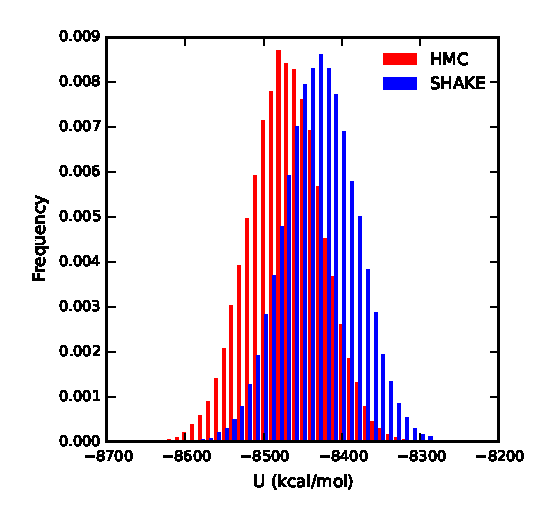
\includegraphics{potenergy}
\end{figure}

\begin{figure}
    \caption{$\timestep$ = 1 fs ($\bar{T}$ = 300.04 K, $\bar{U}$ = -8465.63 kcal/mol)}
	\includegraphics{potenergy2}
\end{figure}

\begin{figure}
    \caption{$\timestep$ = 0.5 fs ($\bar{T}$ = 299.99 K, $\bar{U}$ = -8468.19 kcal/mol)}
	\includegraphics{potenergy_05}
\end{figure}

\begin{figure}
    \caption{$\timestep$ = 1 fs ($\bar{T}$ = 299.52 K, $\bar{U}$ = -8470.21 kcal/mol)}
	\includegraphics{potenergy_kamb}
\end{figure}


In Fig.~\ref{fig:checkensemble} we show the result from the linear regression analysis for the potential energies sampled using Eq.~\eqref{eq:trotter_splitting_NHC}.
In figure legends we show the averages temperatures simulated.
It can be seen that the mentioned algorithm generates a distribution consistent with the canonical ensemble, and that is also true for the kinetic energies.
Likewise, in Fig.~\ref{fig:mbdistribution} we observe a good correspondence between the kinetic energy distribution at $T= 304.99 K$ and the corresponding Maxwell-Boltzmann distribution We arrive at the same conclusions for the approach given by Eq.~\eqref{eq:modified_splitting}.

\begin{figure}
	\includegraphics{checkensemble}
	\caption{Linear plot of the log ratio probabilities with the true slope (solid line) and the measured slope from the linear regression analysis (symbols).
Simulation of liquid water using Eq.~\eqref{eq:trotter_splitting_NHC}, $\timestep$ = 1~fs, $\bar{T}_1$ = 296.03~K, $\bar{T}_2$ = 304.99~K.}
	\label{fig:checkensemble}
\end{figure}

\begin{figure}
	\includegraphics{maxwell-botlzamm-paper}
	\caption{Probability distribution of the kinetic energy with sampled values and those calculated with Eq.~\eqref{eq:mb}.
Simulation of liquid water using Eq.~\eqref{eq:trotter_splitting_NHC}, $\timestep$ = 1~fs, $\bar{T}$ = 304.99~K.}
\label{fig:mbdistribution}
\end{figure}

Finally, in Table~\ref{table:ensemblevalidation} we present the results of the maximum likelihood approach applied for both NVT integration schemes.
It can be seen that the deviations from the true slope, $\timestep$ = 8.970~K, are less than $1\sigma$.
This means that effectively, the sampled values do not deviate from the correct distribution to a statistically noticeable level.

\begin{table}
	\begin{threeparttable}
		\caption{Ensemble Validation of NVT algorithms for liquid water using the Maximum Likelihood Approach \tnote{a} \tnote{b}}
		\label{table:ensemblevalidation}
%		\begin{ruledtabular}
			\begin{tabular}{ccccc}
				& \multicolumn{4}{c}{true $\timestep$ = 8.970 K} \\
				\cline{2-5}
				& \multicolumn{2}{c}{potential} & \multicolumn{2}{c}{kinetic}\\
				\hline
				Method  &$\timestep/K$ & $\sigma$ dev & $\timestep/K$ & $\sigma$ dev \\
				\hline % inserts single-line 
				Eq.~\eqref{eq:trotter_splitting_NHC} & 9.022 $\pm$ 0.117 & 0.57 & 8.928 $\pm$ 0.051 & 0.63 \\
				Eq.~\eqref{eq:modified_splitting}    & 8.965 $\pm$ 0.101 & 0.05 & 8.967 $\pm$ 0.052 & 0.14
		\end{tabular}
%		\end{ruledtabular}
		\begin{tablenotes}
			\item[a] The standard deviation of the mean temperature for all cases is $\sigma$ = 0.03.
			\item[b] $\bar{T}_1$ = 296.03~K and $\bar{T}_2$ = 304.99~K.
		\end{tablenotes}
	\end{threeparttable}
\end{table}

%\begin{center}
%  \label{fig:pressure}
%  \includegraphics{pressure2}
%  \captionof{figure}{Histograms of pressure obtained in this work (filled bars) and using LAMMPS %(unfilled bars).
%Simulation of liquid water with NVE integration.
%$\timestep : 1 fs$  }
%\end{center}


\section{Concluding Remarks}
\label{sec:conclusion}
Nevertheless, as will be shown in the forthcoming section, those numerical schemes successfully achieve the specified temperature and an acceptable long-term conservation of the extended energy $H$.

by contrast

\begin{acknowledgement}
	The authors acknowledge the financial support provided by Petrobras (project code CENPES 16113).
\end{acknowledgement}

\appendix

\bibliography{rigid_bodies}
%\begin{table*}
%	\caption{Results with Exact Solution for Free Rotations}
%	\label{table:NVE}
%	\begin{ruledtabular}
%		\begin{tabular}{cccccccc}
%			$\timestep$ (fs) & $T$ (K) & $\langle U\rangle$ (kcal/mol) & $\langle K\rangle$ (kcal/mol) & $\langle K_t\rangle$ (kcal/mol) & $\langle K_r\rangle$ (kcal/mol) & P (atm) & $R$ (kcal/mol.ns) \\
%			\hline
%			1.0 & $	305.91	\pm	0.03	$ & $	-8395.1	\pm	0.1	$ & $	1645.9	\pm	0.1	$ & $	823.2	\pm	0.1	$ & $	822.7	\pm	0.1	$ & $	146	\pm	2	$ & $0.0456$ \\
%			2.0 & $	305.21	\pm	0.02	$ & $	-8389.5	\pm	0.1	$ & $	1642.1	\pm	0.1	$ & $	823.0	\pm	0.1	$ & $	819.1	\pm	0.1	$ & $	149	\pm	2	$ & $0.656$ \\
%			3.0 & $	304.30	\pm	0.03	$ & $	-8375.4	\pm	0.9	$ & $	1637.2	\pm	0.1	$ & $	824.0	\pm	0.1	$ & $	813.3	\pm	0.1	$ & $	156	\pm	2	$ & $2.87$ \\
%			4.0 & $	304.5	\pm	0.5	$ & $	-8339	\pm	6	$ & $	1638	\pm	3	$ & $	829	\pm	1	$ & $	808.8	\pm	0.6	$ & $	180	\pm	2	$ & $10.1$ \\
%		\end{tabular}
%	\end{ruledtabular}
%\end{table*}

%\begin{table*}
%\caption{Results.....}
%\label{table:NVE}
%\begin{ruledtabular}
%\begin{tabular}{cccccccc}
%$\timestep$ (fs) & $T$ (K) & $\langle U\rangle$ (kcal/mol) & $\langle K\rangle$ (kcal/mol) & $\langle K_t\rangle$ (kcal/mol) & $\langle K_r\rangle$ (kcal/mol) & P (atm) & $R$ (kcal/mol.ns) \\
%\hline
%1.0 & $305.95\pm0.03$ & $-8395.4\pm0.1$ & $1646.1\pm0.1$ & $823.3\pm0.1$ & $822.9\pm0.1$ & $151\pm2$ & $0.0471$ \\
%2.0 & $305.17\pm0.03$ & $-8389.0\pm0.1$ & $1641.9\pm0.1$ & $823.2\pm0.1$ & $818.8\pm0.1$ & $148\pm2$ & $0.853$ \\
%3.0 & $304.34\pm0.03$ & $-8374\pm2$ & $1637.5\pm0.2$ & $824.0\pm0.1$ & $813.4\pm0.1$ & $152\pm2$ & $3.96$ \\
%4.0 & $303.6\pm0.4$ & $-8349\pm5$ & $1633\pm2$ & $826.8\pm0.2$ & $806.5\pm0.4$ & $168\pm2$ & $8.25$ \\
%\end{tabular}
%\end{ruledtabular}
%\end{table*}
%\begin{table}
%	\begin{threeparttable}
%		\caption{Average deviation of the conserved quantity ($DE$) and average temperatures from liquid water simulation with NVT integration \tnote{a}\tnote{b}}
%		\label{table:denvt}
%		\begin{ruledtabular}
%			\begin{tabular}{ccccc}
%				& \multicolumn{2}{c}{Eq.~\eqref{eq:trotter_splitting_NHC}} & \multicolumn{2}{c}{Eq.~%\eqref{eq:modified_splitting}} \\
%				\cline{2-5}
%				$\timestep$/fs & $D\!E$ & $T$/K & $D\!E$ & $T$/K \\
%				\hline
%				1.0 & 0.000043 & 298.16  & 0.000052  & 298.15 \\
%				2.0 & 0.00013  & 298.23  & 0.00017   & 298.06 \\
%				3.0 & 0.00089  & 298.17  & 0.0013    & 298.12
%			\end{tabular}
%		\end{ruledtabular}
%		\begin{tablenotes}
%			\item[a] The standard deviation of the mean temperature for all cases is $\sigma = 0.037$.
%			\item[b] The smaller time step in the NHC and NHC* operators is 0.25 fs.
%		\end{tablenotes}
%	\end{threeparttable}
%\end{table}

%The Nos\'e-Hoover chain propagator is further split by making $i\!L_\text{NHC} = \sum_{j=0}^M i\!L_%\text{NHC}^{(j)}$ and, afterwards,
%\begin{equation*}
%e^{\frac{\timestep}{2} i\!L_\text{NHC}} = \Pi_{j=1}^n \Bigg[ \prod_{j=M}^1 e^{\frac{\timestep}{4} i\!L_\text{NHC}^{(j)} } \Bigg] e^{\frac{\timestep}{2} i\!L_\text{NHC}^{(0)} } \Bigg[ \prod_{j=1}^M e^{\frac{\timestep}{4} i\!L_\text{NHC}^{(j)} } \Bigg].
%\end{equation*}

%In order to satisfy the criterion in Eq.~\eqref{eq:split_kappa_w} for all factors, given the function $w$ expressed in Eq.~\eqref{eq:nhc_measure}, we further split the NHC contribution as $i\!L_\text{NHC} = \sum_{j=0}^M i\!L_\text{NHC}^{(j)}$, where

%\begin{subequations}
%\label{eq:solution_momenta}
%\begin{align}
%&{\vt p}_i(t) = {\vt p}_i^0 + \left({\vt F}_i - \alpha_1 {\vt p}_i^0 \right) \phi\left(\alpha_1 t \right) %t \quad \text{and} \label{eq:solution_p} \\
%&{\vt \pi}_i(t) = {\vt \pi}_i^0 + \left(2 {\mt C}_i{\vt \tau}_i - \alpha_1 {\vt \pi}_i^0 \right) \phi%\left(\alpha_1 t \right) t.
\label{eq:solution_pi}
%\end{align}
%\end{subequations}

%By evaluating these functions simultaneously for all $i$, we accomplish the effect of a propagator $e^{t i%\!L_b^\ast}$, where $i\!L_b^\ast$ is the Liouville operator given by
%\begin{equation*}
%i\!L_b^\ast = \sum_{i=1}^N \left[ \left( \tr{\vt F}_i - \alpha_1 \tr{\vt p}_i \right) \diff{}{\vt p_i} + \left(2 \tr{\vt \tau}_i \tr{\mt C}_i - \alpha_1 \tr{\vt \pi}_i \right) \diff{}{\vt \pi_i} \right].
%\end{equation*}
%We also define a modified Nos\'e-Hoover chain propagator $e^{i\!L^\ast_\text{NHC}}$, as follows:
%\begin{equation}
%\begin{split}
%e^{\frac{\timestep}{2} i\!L_\text{NHC}^\ast } = &\prod_{j=M}^1 \exp\left[\frac{\timestep}{4} \left( G_j - \alpha_{j+1} p_{\eta_j} \right) \diff{}{p_{\eta_j}}\right] \\
%\times &\exp\left(-\frac{\timestep}{2} \sum_{j=1}^M \alpha_j \diff{}{\eta_j}\right) \\
%\times &\prod_{j=1}^M \exp\left[\frac{\timestep}{4} \left( G_j - \alpha_{j+1} p_{\eta_j} \right) \diff{}{p_{\eta_j}}\right]
%\end{split}
%\end{equation}

%In order to evaluate the stability of the numerical integrators, we employ a measure given by%\cite{Tuckerman_2010}
%\begin{equation}
%\label{eq:performance}
%D\!E =  \frac{1}{\mathcal N} \sum_{t=1}^{\mathcal N} \left| \frac{E_t - E_0}{E_0} \right|,
%\end{equation}
%from which it is possible to quantify the average deviation of the supposedly conserved quantity $E$ %(either $\mathcal{H}$ of Eq.~\eqref{eq:H_NVE} or $H$ of Eq.~\eqref{eq:H_nvt}) from its initial value $E_0$ %after a certain number of time steps $\mathcal N$.
% \textbf{In order to use a constant value for the smaller time step in the NHC and NHC* operators $(\timestep/4)$, we factorized those operators analogously to the scheme given by Eq.~\eqref{eq:splitting_rot}}.



%\begin{equation}
%\label{eq:probability_ratio_pot}
%\frac{P_{pot}(E/\beta_2)}{P_{pot}(E/\beta_1)} = \frac{Q_{pot}(\beta_1)}{Q_{pot}(\beta_2)}  \exp\left[(-\beta_2 - \beta_1)E_{pot}\right]
%\end{equation}

%\begin{equation}
%\label{eq:probability_ratio_kin}
%\frac{P_{kin}(E/\beta_2)}{P_{kin}(E/\beta_1)} = \frac{Q_{kin}(\beta_1)}{Q_{kin}(\beta_2)}  \exp\left[(-%\beta_2 - \beta_1)E_{kin}\right]
%\end{equation}

%The equation above avoids the introduction of a ficticious angular velocity component, as required in the formulation of Miller~\textit{et al.}\cite{Miller_2002} An important feature of this relation is that it preserves the unit-norm constraint of a quaternion upon infinitesimal rotation.
\end{document}
